% this is a simplified version of 
% https://github.com/yihui/knitr/blob/master/inst/examples/knitr-beamer.Rnw
\documentclass{beamer}\usepackage[]{graphicx}\usepackage[]{color}
%% maxwidth is the original width if it is less than linewidth
%% otherwise use linewidth (to make sure the graphics do not exceed the margin)
\makeatletter
\def\maxwidth{ %
  \ifdim\Gin@nat@width>\linewidth
    \linewidth
  \else
    \Gin@nat@width
  \fi
}
\makeatother

\definecolor{fgcolor}{rgb}{0.345, 0.345, 0.345}
\newcommand{\hlnum}[1]{\textcolor[rgb]{0.686,0.059,0.569}{#1}}%
\newcommand{\hlstr}[1]{\textcolor[rgb]{0.192,0.494,0.8}{#1}}%
\newcommand{\hlcom}[1]{\textcolor[rgb]{0.678,0.584,0.686}{\textit{#1}}}%
\newcommand{\hlopt}[1]{\textcolor[rgb]{0,0,0}{#1}}%
\newcommand{\hlstd}[1]{\textcolor[rgb]{0.345,0.345,0.345}{#1}}%
\newcommand{\hlkwa}[1]{\textcolor[rgb]{0.161,0.373,0.58}{\textbf{#1}}}%
\newcommand{\hlkwb}[1]{\textcolor[rgb]{0.69,0.353,0.396}{#1}}%
\newcommand{\hlkwc}[1]{\textcolor[rgb]{0.333,0.667,0.333}{#1}}%
\newcommand{\hlkwd}[1]{\textcolor[rgb]{0.737,0.353,0.396}{\textbf{#1}}}%
\let\hlipl\hlkwb

\usepackage{framed}
\makeatletter
\newenvironment{kframe}{%
 \def\at@end@of@kframe{}%
 \ifinner\ifhmode%
  \def\at@end@of@kframe{\end{minipage}}%
  \begin{minipage}{\columnwidth}%
 \fi\fi%
 \def\FrameCommand##1{\hskip\@totalleftmargin \hskip-\fboxsep
 \colorbox{shadecolor}{##1}\hskip-\fboxsep
     % There is no \\@totalrightmargin, so:
     \hskip-\linewidth \hskip-\@totalleftmargin \hskip\columnwidth}%
 \MakeFramed {\advance\hsize-\width
   \@totalleftmargin\z@ \linewidth\hsize
   \@setminipage}}%
 {\par\unskip\endMakeFramed%
 \at@end@of@kframe}
\makeatother

\definecolor{shadecolor}{rgb}{.97, .97, .97}
\definecolor{messagecolor}{rgb}{0, 0, 0}
\definecolor{warningcolor}{rgb}{1, 0, 1}
\definecolor{errorcolor}{rgb}{1, 0, 0}
\newenvironment{knitrout}{}{} % an empty environment to be redefined in TeX

\usepackage{alltt}
\IfFileExists{upquote.sty}{\usepackage{upquote}}{}
\begin{document}

\title{Introducci\'on a la Gen\'omica \\ UNAL nov 2017}
\author{Alejandro Caceres \\ ISGlobal, Barcelona}


\maketitle

% very important to use option [fragile] for frames containing code output!
\begin{frame}[fragile]
\frametitle{Metodos Multidimensionales}
los que mas destacan son el an\'alis de compontentes principales (PCA) y el escalamiento multidimensional (MDS)
\begin{itemize}
\item Miden la variabilidad gen\'etica en una muestra de individuos
\item Determinan la distancia genetic antre poblaciones
\item Se pueden usar para determinar ancestr\'ia 
\end{itemize}
\end{frame}

\begin{frame}[fragile]
\frametitle{Analisis de Componentes Principales}

\begin{figure}[htbp]
\begin{center}
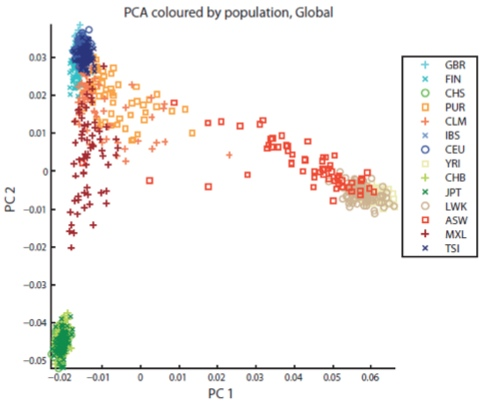
\includegraphics[width=.5\linewidth]{pca1000g.jpg}
\end{center}
\end{figure}
\end{frame}



\begin{frame}[fragile]
\frametitle{Analisis de Componentes Principales}

\begin{figure}[htbp]
\begin{center}
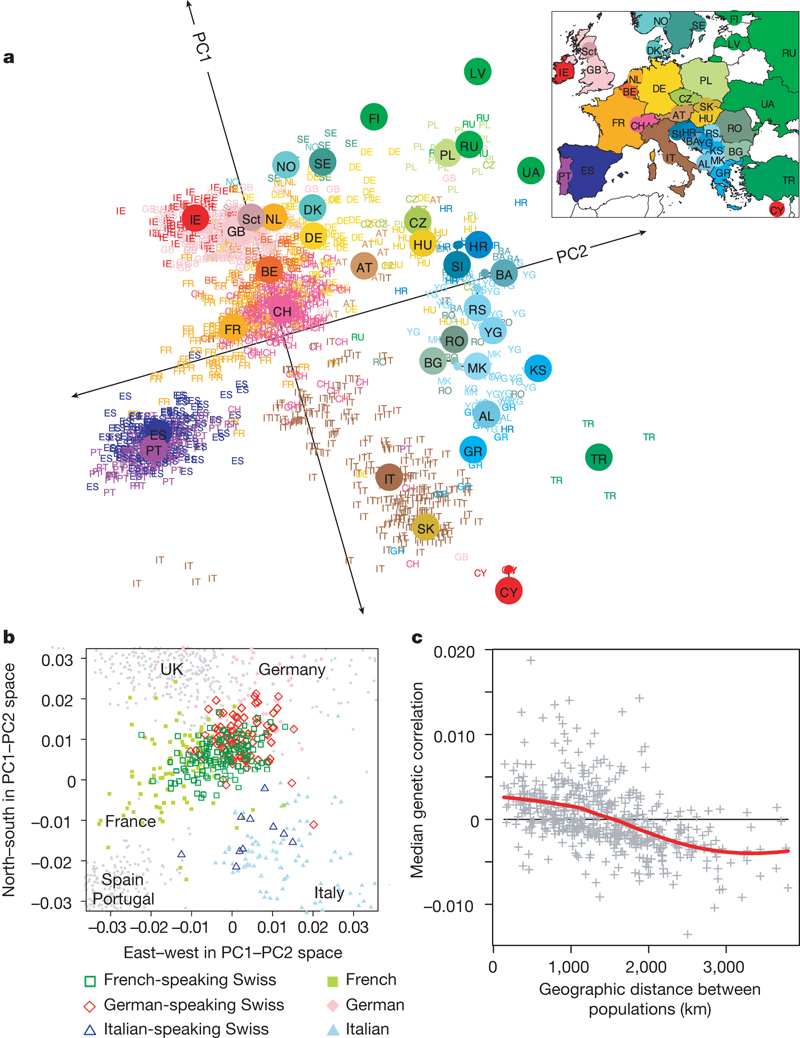
\includegraphics[width=.5\linewidth]{eurpca.jpeg}
\end{center}
\end{figure}
\end{frame}

\begin{frame}[fragile]
\frametitle{Metodos Multidimensionales}

Producen variables que son combinaciones lineales de los SNPs de tal forma que
\begin{itemize}
\item explican la mayor variabilidad posible (PCA). SNPstats and PLINK
\item explican la mayor distancia posible entre individios (MDS). PLINK
\end{itemize}

El n\'umero de variables que se calculan detende de que tanto queramos explicar los datos.

\end{frame}


\begin{frame}[fragile]
\frametitle{snpStats}
Veamos como se calcula PCA en SNPstats
\begin{knitrout}\footnotesize
\definecolor{shadecolor}{rgb}{0.969, 0.969, 0.969}\color{fgcolor}\begin{kframe}
\begin{alltt}
\hlkwd{library}\hlstd{(snpStats)}
\end{alltt}
\end{kframe}
\end{knitrout}
\begin{knitrout}\footnotesize
\definecolor{shadecolor}{rgb}{0.969, 0.969, 0.969}\color{fgcolor}\begin{kframe}
\begin{alltt}
\hlkwd{load}\hlstd{(}\hlstr{"datos/NewsnpsSNPstats.RData"}\hlstd{)}
\hlstd{xxmat} \hlkwb{<-} \hlkwd{xxt}\hlstd{(NewsnpsSNPstats)}
\hlstd{evv} \hlkwb{<-} \hlkwd{eigen}\hlstd{(xxmat)}
\hlstd{pcs} \hlkwb{<-} \hlstd{evv}\hlopt{$}\hlstd{vectors[,}\hlnum{1}\hlopt{:}\hlnum{2}\hlstd{]}
\hlkwd{plot}\hlstd{(pcs)}
\end{alltt}
\end{kframe}
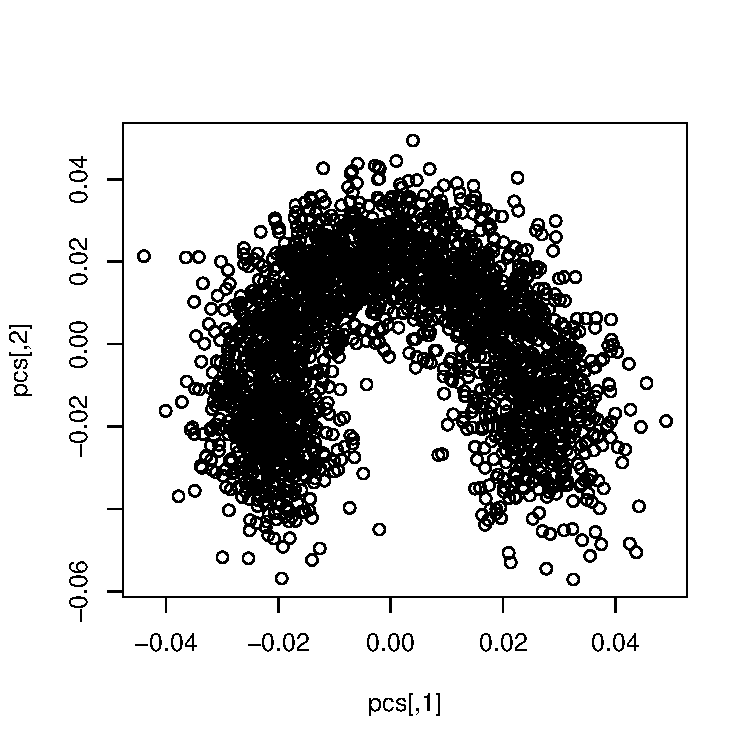
\includegraphics[width=.45\linewidth]{figure/plot1-1} 

\end{knitrout}
el c\'alculo de PCA tarda mucho si son datos de todo el genoma. 
\end{frame}


\begin{frame}[fragile]
\frametitle{snpStats}
Podemos ver que para esta regi\'on el PCA discrimina poblaciones
\begin{knitrout}\footnotesize
\definecolor{shadecolor}{rgb}{0.969, 0.969, 0.969}\color{fgcolor}\begin{kframe}
\begin{alltt}
\hlstd{ids}\hlkwb{<-}\hlkwd{read.table}\hlstd{(}\hlstr{"datos/20130606_g1k.ped"}\hlstd{,} \hlkwc{sep}\hlstd{=}\hlstr{"\textbackslash{}t"}\hlstd{,} \hlkwc{header}\hlstd{=}\hlnum{TRUE}\hlstd{)}

\hlkwd{rownames}\hlstd{(ids)}\hlkwb{<-}\hlstd{ids}\hlopt{$}\hlstd{Individual.ID}
\hlstd{pops}\hlkwb{<-}\hlstd{ids[}\hlkwd{rownames}\hlstd{(NewsnpsSNPstats),]}\hlopt{$}\hlstd{Population}

\hlkwd{plot}\hlstd{(pcs,} \hlkwc{col}\hlstd{=}\hlkwd{as.numeric}\hlstd{(pops),} \hlkwc{pch}\hlstd{=}\hlnum{16}\hlstd{)}
\hlkwd{legend}\hlstd{(}\hlstr{"topright"}\hlstd{,} \hlkwc{legend}\hlstd{=}\hlkwd{levels}\hlstd{(pops),} \hlkwc{pch}\hlstd{=}\hlnum{16}\hlstd{,} \hlkwc{col}\hlstd{=}\hlnum{1}\hlopt{:}\hlkwd{length}\hlstd{(}\hlkwd{levels}\hlstd{(pops)),} \hlkwc{cex}\hlstd{=}\hlnum{0.7}\hlstd{)}
\end{alltt}
\end{kframe}
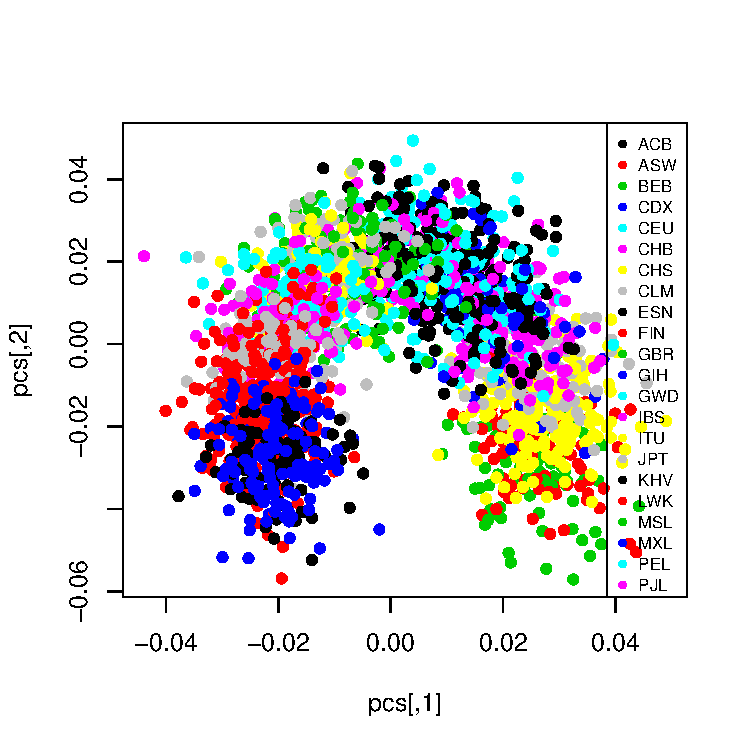
\includegraphics[width=.45\linewidth]{figure/plot2-1} 

\end{knitrout}

\end{frame}


\begin{frame}[fragile]
\frametitle{PLINK}

Debido a que los analisis multivariantes son constosos computacionalmente es mejor usar codigo compilado
PLINK.

\begin{verbatim}
plink --bfile  mydata --pca --out mydata
plink --bfile  mydata --mds-plot --out mydata --neighbour 1 15
\end{verbatim}
Los resultados deben ser muy similares.
--neighbour 1 15 calcula las distancias del primer al 15 vecinos mas cercanos para determinar si un individuo es un outlier 
en terminos de ancestr\'ia 

\end{frame}

\end{document}
